%% Total contracts = 367
%% Total checks = 181182
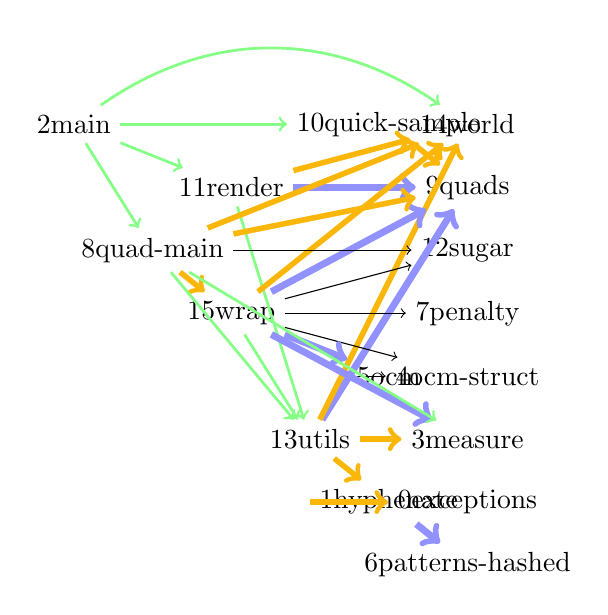
\begin{tikzpicture}

  \node (00)               {\rkt{14}{world}};
  \node (01) [below of=00,yshift=0.2cm] {\rkt{9}{quads}};
  \node (02) [below of=01,yshift=0.2cm] {\rkt{12}{sugar}};
  \node (03) [below of=02,yshift=0.2cm] {\rkt{7}{penalty}};
  \node (04) [below of=03,yshift=0.2cm] {\rkt{4}{ocm-struct}};
  \node (05) [below of=04,yshift=0.2cm] {\rkt{3}{measure}};
  \node (06) [below of=05,yshift=0.2cm] {\rkt{0}{exceptions}};
  \node (07) [below of=06,yshift=0.2cm] {\rkt{6}{patterns-hashed}};

  \node (10) [left of=00] {\rkt{10}{quick-sample}};
  \node (11) [left of=01] {};
  \node (12) [left of=02] {};
  \node (13) [left of=03] {};
  \node (14) [left of=04] {\rkt{5}{ocm}};
  \node (15) [left of=05] {};
  \node (16) [left of=06] {\rkt{1}{hyphenate}};

  \node (20) [left of=10] {};
  \node (21) [left of=11] {};
  \node (22) [left of=12] {};
  \node (23) [left of=13] {};
  \node (24) [left of=14] {};
  \node (25) [left of=15] {\rkt{13}{utils}};

  \node (30) [left of=20] {};
  \node (31) [left of=21] {\rkt{11}{render}};
  \node (32) [left of=22] {};
  \node (33) [left of=23] {\rkt{15}{wrap}};
  \node (35) [left of=25] {};

  \node (40) [left of=30] {};
  \node (42) [left of=32] {\rkt{8}{quad-main}};
  \node (45) [left of=35] {};

  \node (50) [left of=40] {\rkt{2}{main}};

  %% -- edges
  %% hyphenate
  \draw[->,yellow!45!orange, line width=2pt] (16) -- (06);
  \draw[->,blue!43!white, line width=2.5pt] (16) -- (07);
  %% quick-sample
  \draw[->,yellow!45!orange, line width=2pt] (10) -- (01);
  %% ocm
%% WARNING: no data for boundary 'ocm-struct.rkt' ==> 'ocm.rkt'
  \draw[->] (14) -- (04);
  %% utils
  \draw[->,yellow!45!orange, line width=2pt] (25) -- (16);
  \draw[->,yellow!45!orange, line width=2pt] (25) -- (05);
  \draw[->,blue!43!white, line width=2.5pt] (25) -- (01);
  \draw[->,yellow!45!orange, line width=2pt] (25) -- (00);
  %% render
  \draw[->,yellow!45!orange, line width=2pt] (31) -- (00);
  \draw[->,blue!43!white, line width=2.5pt] (31) -- (01);
  \draw[->,green!48!white, line width=1pt] (31) -- (25);
  %% wrap
  \draw[->,yellow!45!orange, line width=2pt] (33) -- (00);
  \draw[->,blue!43!white, line width=2.5pt] (33) -- (01);
%% WARNING: no data for boundary 'sugar.rkt' ==> 'wrap.rkt'
  \draw[->] (33) -- (02);
%% WARNING: no data for boundary 'penalty.rkt' ==> 'wrap.rkt'
  \draw[->] (33) -- (03);
%% WARNING: no data for boundary 'ocm-struct.rkt' ==> 'wrap.rkt'
  \draw[->] (33) -- (04);
  \draw[->,blue!43!white, line width=2.5pt] (33) -- (05);
  \draw[->,blue!43!white, line width=2.5pt] (33) -- (14);
  \draw[->,green!48!white, line width=1pt] (33) -- (25);
  %% quad-main
  \draw[->,yellow!45!orange, line width=2pt] (42) -- (00);
  \draw[->,yellow!45!orange, line width=2pt] (42) -- (01);
  \draw[->,yellow!45!orange, line width=2pt] (42) -- (33);
  \draw[->,green!48!white, line width=1pt] (42) -- (05);
  \draw[->,green!48!white, line width=1pt] (42) -- (25);
%% WARNING: no data for boundary 'sugar.rkt' ==> 'quad-main.rkt'
  \draw[->] (42) -- (02);
  %% main
  \draw[->,green!48!white, line width=1pt] (50) edge[bend left=35] (00);
  \draw[->,green!48!white, line width=1pt] (50) -- (42);
  \draw[->,green!48!white, line width=1pt] (50) -- (10);
  \draw[->,green!48!white, line width=1pt] (50) -- (31);

\end{tikzpicture}
